\section{Semantics of Differential Datalog}\label{sec:ddlog}\label{sec:datalog}

This section gives a semantics of DDlog in terms of \dbsp circuits.
This is a precise specification of the semantics of DDlog.

\subsection{Differential Datalog syntax and semantics}\label{sec:datalog-syntax}

We describe the syntax and semantics of a dialect of Datalog called Differential Datalog,
or DDlog.  We start by ignoring the differential aspects, we will return to these in Section~\ref{sec:ddlog}.
In defining the syntax and semantics of Datalog we mostly follow standard definitions, e.g.,~\cite{Abiteboul-book95}.
In this section we give a syntax-directed translation of Datalog programs into circuits.
We model a \emph{core} of the language (ignoring constructs that can be viewed as syntactic sugar), 
to simplify the description.  We argue informally that the resulting circuits implement the standard
semantics of Datalog.

\begin{figure}[t]
{\small
\begin{lstlisting}[numbers=left]
DatalogProgram := TypeDeclaration*
                  RelationDeclaration* 
                  Rule*
TypeDeclaration := ...
Type := ...
Expression := ...
Id := ... // identifiers
RelationDeclaration := ("input"|"output")? "relation"
                       Id "(" ColumnTypes? ")"
ColumnTypes := ColumnType ( "," ColumnType)*
ColumnType := Id ":" Type
Rule := Head ":-" Body
Head := RelationTerm
RelationTerm := Id "(" Columns? ")"
Columns := Variable ( "," Variable )*
Body := RelationTerm ( "," Term )?
Term := RelationTerm 
     | Predicate 
     | NegatedTerm 
     | VariableDefinitionTerm
     | FlatmapTerm
     | GroupByTerm
NegatedTerm := "not" RelationTerm
VariableDefinitionTerm := "var" Variable "=" Expression
FlatmapTerm := "var" Variable "=" "Flatmap" "(" Id ")"
GroupByTerm := "var" Variable "=" 
     Expression "." "group_by" "(" VariableList? ")"
Variable := Id     
VariableList := Id (, Id)*
Predicate := Expression
\end{lstlisting}
}
\caption{Datalog rules grammar.\label{fig:grammar}}
\end{figure}

Our Datalog is strongly-typed, supports stratified negation and recursion, and
is enhanced with additional operators, such as grouping (which we will describe below).
Figure~\ref{fig:grammar} shows the EBNF-like grammar of the core DDlog language
(omitting types and expressions).

\paragraph{Types}

Assume that we are given a set of basic types, including \code{integer}, Booleans, \code{string}, 
but also structures (product types), unions (sum types), tuples, vectors, and sets.
Each such type must support an operation to compare values for equality.  This is the only
requirement to store values of a particular type in a set.

We allow arbitrary computations over the base types (e.g., arithmetic) through the use of
built-in functions (e.g., addition, subtraction, equality comparison, etc.).  A standard
language of expressions can be used to combine built-in functions into more complex
functions.  We require all such functions to be total and deterministic.
We treat such computations as uninterpreted functions (black boxes) and no longer
concern ourselves with them in this document.

All DDlog programs must be strongly typed, but we don't specify the typing rules in
this document (e.g., predicates must produce Boolean results).  
The typing rules are standard.  Only the semantics of well-typed
programs is defined.

\paragraph{Relations}

Datalog programs compute over relations.  The inputs and outputs of a Datalog
program are relations.  The standard Datalog semantics of 
a relation is a \emph{set} of values from some domain.

DDlog programs continuously interact with their environment.  Thus they 
distinguish relations by their roles.  Some relations are \code{input} relations;
their contents is supplied by the environment.  Some relations
are declared as \code{output} relations.  The contents of these relations is visible
to external observers.

A DDlog program must have a declaration for each relation, specifying
the type of its elements, as in this example:

\begin{lstlisting}[language=ddlog]
input relation People(name: string, age: integer)
relation Ages(age: integer)
output relation Names(name: string)
\end{lstlisting}

This declares three relations.  The first relation is an \code{input} relation, named \code{People},
and it has 2 columns, \code{name} of type \code{string}, and \code{age} of type \code{integer}.
Its elements are 2-tuples of type (\code{string}, \code{integer}).  

The value of relation \code{People} is a \emph{set} of such tuples.  As a running example,
let us assume that the input relation \code{People} has the value (supplied by the
program's environment) $\{ (\code{bob}, 10), 
(\code{john}, 20), (\code{amy}, 10) \}$, containing three tuples.  

The relation \code{Names} has a single column, and it is an \code{output} relation.
This means that the environment can observe it's contents.  The relation \code{Ages}
is neither \code{input} nor \code{output}.  The Datalog program must contain
\emph{rules} that show how \code{Ages} and \code{Names} are
computed from the \code{input} relations, i.e., \code{People}.

\paragraph{Rules}

Besides type and relation declarations, the most important part of a Datalog program is a set of rules.
A \defined{Datalog rule} defines the contents of a relation as a function 
of other relations.  A rule has a \defined{head} and a \defined{body}, as shown in the
grammar from Figure~\ref{fig:grammar}.  In the following rule:

\noindent
\begin{lstlisting}[language=ddlog]
Names(n) :- People(n, a).
\end{lstlisting}

\noindent the head is to the left of the turnstyle symbol \code{:-},
and it is always a relation with variables standing for the tuple fields.
This rule defines how \code{Names} is computed from the contents
of \code{People}.
In this example the rule's head is \code{Names(n)}.  
You may guess that the value of \code{Names} is the set 
$\{ \code{bob}, \code{john}, \code{amy} \}$.  We will explain how this result is computed.
The turnstyle symbol can be read as ``if''.
\code{n} is a variable of type \code{string}, standing for the column \code{name}
(the type of \code{n} is \code{string} because it stands positionally for the declared
column \code{name} with type \code{string} of relation \code{Names}).
The values that \code{n} may take are defined by the body of the rule
--- each variable in the head must appear in the body of the rule.

The body of a rule consists of one or two \defined{terms} separated by commas;
a comma is read as an ``and'', and such a rule is form of a \emph{conjunctive query}.
The valuation computed by the body is defined recursively on the list of terms
in the body.  Datalog allows an arbitrary number of terms in a rule body,
but our grammar allows only two.  We argue in the paragraph below that
this does not reduce the power of the language, but it simplifies the
description.

The grammar of terms is shown in line 16 in Figure~\ref{fig:grammar}.  We will discuss
the semantics of the various terms and their implementation as circuits in the rest of this section.

\paragraph{Valuations}

The body of the above rule is \code{People(n, a)}.  The body defines
two variables, \code{n} and \code{a}.
The semantics of a rule body is a \defined{valuation}: 
a set of values that the variables defined by the body may \emph{jointly} take.
Our example body defines a valuation for the tuple of variables (\code{n}, \code{a}).
Since the body is \code{People(n,a)}, the valuation defines the set of values for $(\code{n},\code{a})$
to be the contents of the relation \code{People}, that is $(\code{n},\code{a}) \in \{ (\code{bob}, 10),
(\code{john},20), (\code{amy}, 10) \}$.

We can assume without loss of generality that every rule body has at most two terms.
A rule with $n$ terms can be decomposed into $n$ - 1 rules with 2 terms each by introducing
a temporary relation that stores the entire valuation.
For example, consider the following rule:

\begin{lstlisting}[language=ddlog]
input relation Lives(name:string, country:string)
output relation USAges(age: integer)
USAges(a) :- People(n, a), Lives(n, c), c == "USA".
\end{lstlisting}

The rule prefix \code{People(n, a), Lives(n, c)} defines a valuation for
variables \code{n, a, c}.  By introducing a temporary relation 
\code{Temp(n, a, c)} we can rewrite this rule as two rules, producing the same
result for the visible relatin \code{USAges}:

\begin{lstlisting}[language=ddlog]
relation Temp(name:string, age:integer, country:string)
Temp(n, a, c) :- People(n, a), Lives(n, c).
USAges(a) :- Temp(n, a, c), country == "USA".
\end{lstlisting}

\subsection{Compiling Datalog programs to circuits}

A Datalog program is a set of rules computing over valuations and relations.
Both relations and valuations are represented as \zrs in a translation to circuits,
by representing each set by a \zr with weights 1.  (Subsequent optimizations can
relax this requirement for internal relations as long as the semantics
of output relations is preserved, since only \code{output}
relations are observable from the environment.  We expand on this
in Section~\ref{sec:optimizations}.)  

\subsubsection{Rule compilation}

Each rule is compiled to a circuit with the following properties:

\begin{itemize}
    \item Each relation and valuation is represented by a \zr.
    \item The head of the rule is the output edge of the circuit;
    \item The relations that appear in the body are inputs of the circuit;
    \item The circuit structure is defined by the terms that appear
    in the relation body (as discussed in the rest of this section);
    \item The turnstyle is compiled into a projection operator (described in 
    Section~\ref{sec:projection});
    \item The \emph{valuation} at a conjunction in the rule body
    is translated into an edge in the circuit, carrying \zr values.
\end{itemize}

This translation is illustrated in Figure~\ref{fig:compilation}.

\begin{figure}[h]
    \center
    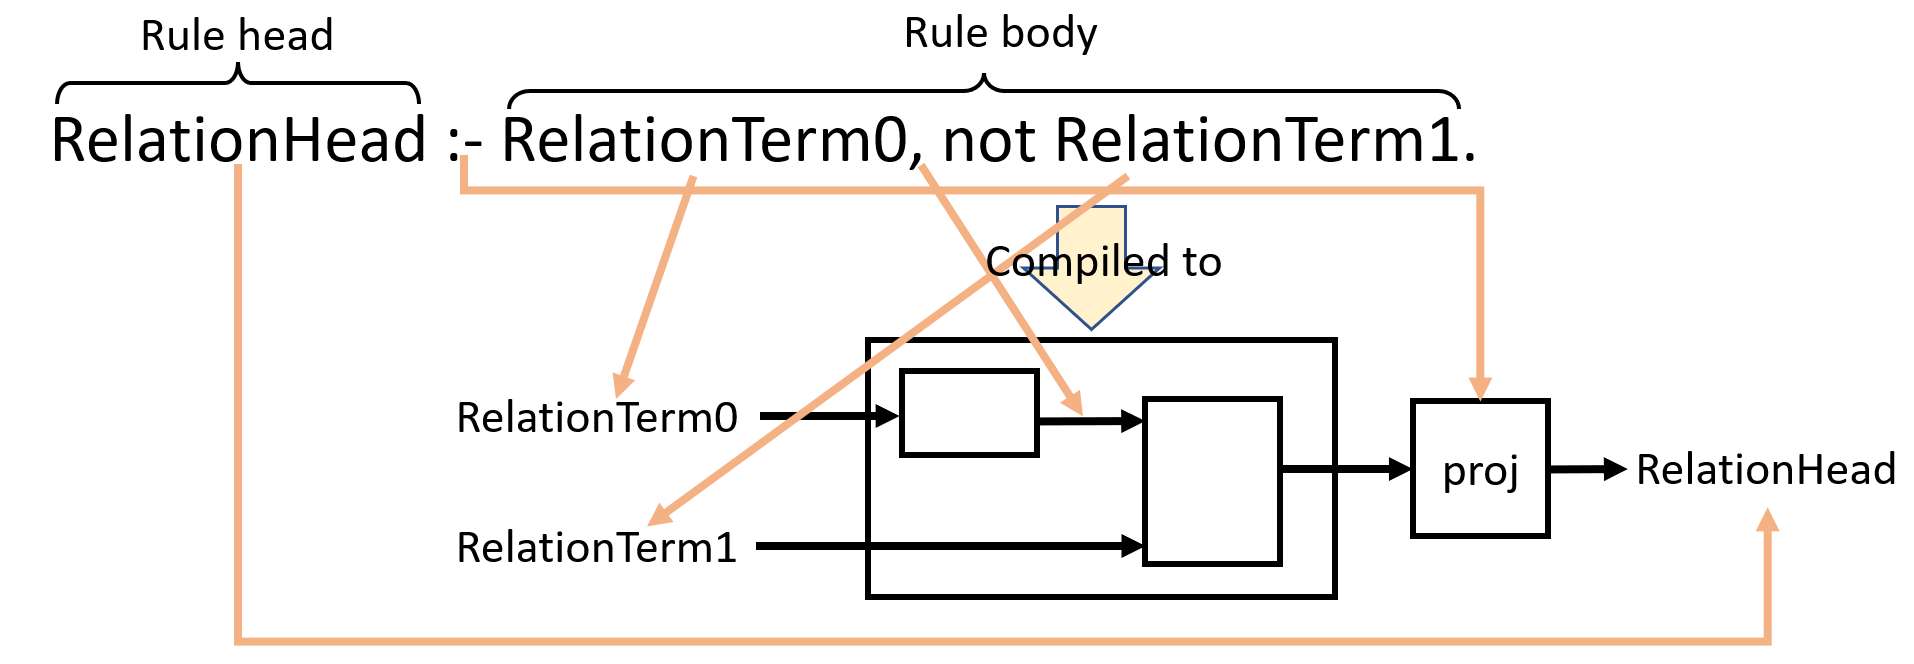
\includegraphics[width=\columnwidth,clip=true]{compilation.png}
    \caption{Compilation of a DDlog rule into a circuit.\label{fig:compilation}}
\end{figure} 

The compilation of a program containing a set of rules produces a ``toplevel'' circuit,
composed of the circuits for the rules interconnected with each other (as described
in Section~\ref{sec:connections}).
For the toplevel circuit the \code{input} relations correspond to the input 
edges.  (\code{input} relations cannot appear in the head of any rule).  Similarly,
the \code{output} relations will correspond to output edges of the toplevel circuit,
(each \code{output} relation must appear in some rule head).

\subsubsection{Relation terms in rule bodies}\label{sec:connections}

A \code{RelationTerm} is a term in a rule body containing a relation with variables substituted 
for the columns: \code{People(n, a)} is such an example.
This term \emph{defines a valuation} for all variables that appear in the columns; 
the valuation associates the variables with the contents of the relation itself.  In our example
the term \code{People(n, a)} defines the following valuation:
$(\code{n}, \code{a}) \in \{ (\code{bob}, 10), (\code{john}, 20), (\code{amy}, 10) \}$.
Each Datalog relation is represented by an edge in a circuit
carrying a \zr.  

As Figure~\ref{fig:compilation} shows, a relation in the head of a rule is compiled into the  
output edge of the circuit corresponding to the rule, and that a \code{RelationTerm}
in the body of a rule is compiled into an input edge of the circuit
corresponding to the rule.

A relation that appears in the body of a rule and in the head of another
rule is compiled into an edge connecting the circuits representing the two rules.
This is in fact just a form of function composition.

(This rule does not apply directly for recursive rules; the translation for recursive
or mutually recursive rules (which define a relation
in terms of itself), is described in Section~\ref{sec:recursion}).

For example, for the following Datalog program structure, where \code{R} is used
within a body and within a separate head:

\begin{lstlisting}[language=ddlog]
R(y) :- I(x), ....
O(y) :- ..., R(y).
\end{lstlisting}

\noindent and, given circuits $C_R$ implementing the first rule and $C_O$
implementing the second rule:

\begin{tikzpicture}[auto,>=latex]
  \node[] (I) {\code{I}};
  \node[block, right of=I] (CR) {$C_R$};
  \node[right of=CR] (R) {\code{R}};
  \draw[->] (I) -- (CR);
  \draw[->] (CR) -- (R);
  
  \node[below of=I] (RI) {\code{R}};
  \node[block, right of=RI] (CO) {$C_O$};
  \node[right of=CO] (O) {\code{O}};
  \draw[->] (RI) -- (CO);
  \draw[->] (CO) -- (O); 
\end{tikzpicture}

\noindent the translation of the program with both rules is:

\begin{tikzpicture}[auto,>=latex]
  \node[] (I) {\code{I}};
  \node[block, right of=I] (CR) {$C_R$};
  \draw[->] (I) -- (CR);
  
  \node[block, right of=R] (CO) {$C_O$};
  \node[right of=CO] (O) {\code{O}};
  \draw[->] (CR) -- node (R) {\code{R}} (CO);
  \draw[->] (CO) -- (O); 
\end{tikzpicture}

This construction is repeated for all rules, translating a program with $n$ rules into
$n$ circuits connected to each other.  If the rules are not recursive the resulting
circuit is acyclic.

\subsubsection{Repeated rule heads (set union)}\label{sec:union}\index{union}

The same relation may appear in the head of multiple rules.
In this case the contents of the head relation is the \emph{set union}
of the values assigned by all heads.
Consider the following example, where \code{I1} and \code{I2} are
rule bodies of arbitrary complexity providing a valuation for variable 
\code{v}:

\begin{lstlisting}[language=ddlog]
O(v) :- I1(v).
O(v) :- I2(v).
\end{lstlisting}

The following circuit implements the Datalog program with both rules:

\begin{tikzpicture}[auto,>=latex]
  \node[] (input1) {\code{I1}};
  \node[below of=input1, node distance=.5cm] (midway) {};
  \node[below of=midway, node distance=.5cm] (input2) {\code{I2}};
  \node[block, shape=circle, right of=midway, inner sep=0in] (plus) {$+$};
  \node[block, right of=plus, node distance=1.5cm] (distinct) {$\distinct$};
  \node[right of=distinct, node distance=1.5cm] (output) {\code{O}};
  \draw[->] (input1) -| (plus);
  \draw[->] (input2) -| (plus);
  \draw[->] (plus) -- (distinct);
  \draw[->] (distinct) -- (output);
\end{tikzpicture}

Given two \zrs $a \in \Z[I]$ and $b \in \Z[I]$
which are sets (i.e., $\isset(a)$ and $\isset(b)$), their \emph{set union} 
can be computed as: $\cup: \Z[I] \times \Z[I] \rightarrow \Z[I]$.  $a
\cup b \defn \distinct(a +_{\Z[I]} b)$.  
The $\distinct$ application is necessary to provide the set semantics of
Datalog.  We have $\isset(a) \land \isset(b) \Rightarrow
\isset(a \cup b)$ and $\ispositive(a) \land \ispositive(b)
\Rightarrow \ispositive(a \cup b)$.

Consider a concrete example for the above program where the value of \code{I1(v)} 
is $\code{v} \in \{ \code{bob} \mapsto 1, \code{mike} \mapsto 1 \}$ and the value of
\code{I2(v)} is $\code{v} \in \{ \code{bob} \mapsto 1, \code{john} \mapsto 1 \}$.
In terms of \zrs we are performing the following addition:

\noindent
\begin{tabular}{ccccc}
\begin{tabular}{|l|l|} \hline
\textbf{\code{v}} & \textbf{W} \\ \hline
\code{bob} & 1 \\
\code{mike} & 1 \\ \hline
\end{tabular} &
$+$ &
\begin{tabular}{|l|l|} \hline
\textbf{\code{v}} & \textbf{W} \\ \hline
\code{bob} & 1 \\
\code{john} & 1 \\ \hline
\end{tabular} &
$=$ &
\begin{tabular}{|l|l|} \hline
\textbf{\code{v}} & \textbf{W} \\ \hline
\code{bob} & 2 \\
\code{mike} & 1 \\
\code{john} & 1 \\ \hline
\end{tabular}
\end{tabular}

It is apparent why the $\distinct$ operator is needed.

\subsubsection{Projection}\label{sec:projection}\index{projection}

Given a valuation produced by the body of a rule, the head of
the rule defines the contents of a relation as \emph{the projection}
of the valuation on the variables used in the head.  For our example rule
\code{Names(n) :- People(n, a)}, the body defines a valuation for $(\code{n}, \code{a})$,
but the head uses only $\code{n}$.
The projection of the valuation $(\code{n}, \code{a}) \in \{ (\code{bob}, 10), (\code{john}, 20), (\code{amy}, 10) \}$
on the variable \code{n} is the valuation
$\code{n} \in \{ \code{bob}, \code{john}, \code{amy} \}$.  This defines
the contents of the relation in the head: $\code{Names} = \{ \code{bob}, \code{john}, \code{amy} \}.$

Thus, in Datalog projection is used when some of the bound variables 
in the body of a rule are not used in the head.  We can assume without loss of 
generality that a single variable is removed in a projection (by bundling multiple
variables in a single tuple-valued variable).  
Let us consider the following example, where \code{I} stands for a rule body producing
a valuation for \code{(v, v1)}.

\begin{lstlisting}[language=ddlog]
O(v) :- I(v, v1).    
\end{lstlisting}

Here the type of the implementation of \code{I} is $\Z[A_0 \times A_1]$ (a \zr of tuples with 
two elements), while the type of the implementation of \code{O} is $\Z[A_0]$.  In terms of \zrs, the
projection of a \zr $i$ on $A_0$ is defined as: $\pi_0(i)[t] = \sum_{x \in i, x|_0 = t} i[x]$, 
where $x|_0$ is first component of the tuple $x$.  The multiplicity of a tuple in the result
is the sum of the multiplicities of all tuples that project to it.

As a concrete example of projection, consider the \zr corresponding to the 
\code{People} relation and it's projection on the \code{Age} column.
The projection is $\pi_{Age}(\code{People}) = \{ 10 \mapsto 1 + 1, 20 \mapsto 1 \}$.
Notice that in the projection the weight of 10 is the sum of all weight of
the tuples that have age 10, i.e., 2.

The circuit for such a rule is:

\begin{tikzpicture}[auto,>=latex]
  \node[] (input) {\code{I}};
  \node[block, right of=input] (pi) {$\pi_0$};
  \node[block, right of=pi, node distance=1.5cm] (distinct) {$\distinct$};
  \node[right of=distinct, node distance=1.5cm] (output) {\code{O}};
  \draw[->] (input) -- (pi);
  \draw[->] (pi) -- (distinct);
  \draw[->] (distinct) -- (output);
\end{tikzpicture}

Note that $\lift{\pi}$ is time-invariant, since $\pi$ has the zero-preservation
property.  We have $\isset(i) \Rightarrow \isset(\pi_A(i))$ and $\ispositive(\pi_0)$.

\subsubsection{Flatmap in DDlog}\label{sec:flatmap} \index{flatmap} 

Recall that in DDlog the type of a column in a relation can be
any of the types supported by the language, including complex types,
such as vectors, sets, or even maps.  For example, the following
declaration indicates that the values in relation \code{I} are 
sets of integers.

\begin{lstlisting}[language=ddlog]
relation I(set: Set<integer>)
\end{lstlisting}

Flatmap is an operator that can expand the data in such a collection value
stored in a relation into the contents of a relation.  Classic Datalog does not support flatmaps. 
In DDlog \code{Flatmap} is an explicit keyword.  It appears
in rules in the form of a \code{FlatmapTerm} in 
the grammar in Figure~\ref{fig:grammar}.  The DDlog type system ensures that the \code{Flatmap} 
operator can only be applied to an expression whose type is a collection.

Here is an example of a program using \code{Flatmap}:

\begin{lstlisting}[language=ddlog]
relation I(set: Set<integer>)
relation O(integer)
O(v) :- I(set), var v = Flatmap(set).
// O = union of all sets in I
\end{lstlisting}

Each element in relation \code{I} is a set of integers.  
The DDlog \code{Flatmap}\index{\code{Flatmap}} operator implements a restricted form of
the functionality of the general mathematical operator from above 
(unlike the mathematical flatmap, which is parameterized by a function $f$, the DDlog
\code{Flatmap} uses a hardwired function, essentially the identity function.).  
The semantics is as follows: the \code{Flatmap} rule body term extends the existing valuation
with a new variable, \code{v} in this example.  \code{Flatmap}'s argument is
an expression that depends on the current valuation (\code{set} in this example)
whose value is a collection.  Let us assume that the contents of the \code{I} relation is: 
$\{ \{1,2\}, \{2,3\} \}$.  

The valuation produced by the rule \code{I(set), var v = Flatmap(set)} is
the following: $(\code{set}, \code{v}) \in  \{ (\{1,2\}, 1), (\{1,2\}, 2), 
(\{2,3\}, 2), (\{2,3\}, 3) \}$.

The circuit-based implementation of \code{Flatmap}, operating on \zrs, can be
defined as follows:

\begin{tikzpicture}[auto,>=latex]
  \node[] (input) {\code{I}};
  \node[block, right of=input, node distance=1.5cm] (map) {$\mbox{flatmap}(e)$};
  \node[block, right of=map, node distance=2cm] (distinct) {$\distinct$};
  \node[right of=distinct, node distance=1.5cm] (output) {\code{O}};
  \draw[->] (input) -- (map);
  \draw[->] (map) -- (distinct);
  \draw[->] (distinct) -- (output);
\end{tikzpicture}

\noindent where the function $e$ extends each tuple in a \zr with the newly introduced variable 
and each set value with a Cartesian product between the collection and all it's elements.
For our example: $e: \code{Set<integer>} \to \Z[\code{Set<integer>} \times \code{integer}]$ 
defined by: $e(\code{set}) = \sum_{x \in \code{set}} (\code{set}, x) \mapsto 1$.

The $\code{distinct}$ operator is needed because some collections (e.g., vectors)
may contain duplicate values.

\begin{proposition}
$\ispositive(\code{Flatmap})$.
\end{proposition}

\subsubsection{Map in DDlog}\label{sec:map}\index{map}

Given a function $f : A \rightarrow B$, the mathematical \defined{map} operator ``lifts'' the
function $f$ to operate on \zrs: $\map(f) : \Z[A] \rightarrow \Z[B]$.
map can be defined in terms of flatmap: $\map(f) \defn \mbox{flatmap}(x \mapsto 1 \cdot f(x))$.

Classic Datalog does not support map computations, but many practical
implementations do.  DDlog programs perform map computations when using \code{VariableDefinitionTerm}
in a rule, by using an expression to computing a value for a new variable, that is added to a valuation,
as in the following example:

\begin{lstlisting}[language=ddlog]
O(v) :- I(x), var v = x + 1. 
\end{lstlisting}

The \code{VariableDefinitionTerm}, \code{var v = x + 1}, extends the current valuation, which
contains just \code{x}, to include the newly defined variable \code{v}.  

The circuit implementation of the previous rule is:

\begin{tikzpicture}[auto,>=latex]
  \node[] (input) {\code{I}};
  \node[block, right of=input, node distance=1.5cm] (map) {$\mbox{map}(e)$};
  \node[right of=map, node distance=1.5cm] (output) {\code{O}};
  \draw[->] (input) -- (map);
  \draw[->] (map) -- (output);
\end{tikzpicture}

The function $e$ extends the current valuation tuple with a new column 
(corresponding to \code{v} in the example) and
evaluates the expression in the term (\code{x + 1}) for each row of the valuation
to compute the corresponding value for the new column.  In our example,
$e: \Z[\code{integer}] \to \Z[\code{integer} \times \code{integer}]$,
$e(x) = (x, x+1)$.

Note that $\ispositive(\map(f))$ for any function $f$.  
From the linearity of flatmap it follows that $\map$
is linear as well.  Moreover, the operator $\lift{\map(f)}$ is
time-invariant for any $f$.

\subsubsection{Filtering}\label{sec:filtering}

Filtering occurs in Datalog whenever a \code{TermPredicate} appears in 
the body of a rule, in the guise of a Boolean expression, as in the following example:

\noindent
\begin{lstlisting}[language=ddlog]
relation Minors(n: string, a: integer)
Minors(n, a) :- People(n, a), a < 18.
\end{lstlisting}

(A predicate may not appear in the first position in the body of a rule.)
The predicate must only use variables in the current valuation.
The produced valuation contains the same variables as the source valuation.
The value of the valuation the set of tuples in the source valuation that 
satisfy the predicate. 

Recall that the valuation of the term \code{People(n, a)} is
$(\code{n}, \code{a}) \in \{ (\code{bob}, 10), \\ (\code{john}, 20), (\code{amy}, 10) \}$.
The valuation of the entire rule is the set of tuples $(\code{n}, \code{a})$
for which the predicate $\code{a} < 18$ holds.  That valuation is
$(\code{n}, \code{a}) \in \{ (\code{bob}, 10), (\code{amy}, 10) \}$.  Thus the contents
of relation $\code{Minors}$ is $\{ (\code{bob}, 10), (\code{amy}, 10) \}$.

To compute on \zrs, let us assume that we are filtering with a predicate $P: A \rightarrow \B$.  
We define the following function $\sigma_P: A \rightarrow \Z[A]$ as:
$$\sigma_P(x) = \left\{
\begin{array}{ll}
  1 \cdot x & \mbox{ if } P(x) \\
  0 & \mbox{ otherwise } \\
\end{array}
\right.
$$

The filter of a \zr is defined as $\mbox{filter}_P: \Z[A]
\rightarrow \Z[A]$ by $\mbox{filter}_P \defn
\mbox{flatmap}(\sigma_P)$.  We have $\isset(i) \Rightarrow
\isset(\mbox{filter}_P(i))$ and $\ispositive(\mbox{filter}_P)$.  Thus a $\distinct$
is not needed.  As a consequence of the linearity of $\mbox{flatmap}$, we have
that filtering is also linear.   The lifted version of filtering is also time-invariant.

The circuit for filtering with a predicate $P$ can be implemented as:

\begin{tikzpicture}[auto,>=latex]
  \node[] (input) {\code{I}};
  \node[block, right of=input, node distance=2cm] (map) {$\mbox{flatmap}(\sigma_P)$};
  \node[right of=map, node distance=2cm] (output) {\code{O}};
  \draw[->] (input) -- (map);
  \draw[->] (map) -- (output);
\end{tikzpicture}

\subsubsection{Grouping}\index{grouping}\label{sec:grouping}

Classic Datalog does not support grouping.
In DDlog grouping is the fundamental operator used for aggregation.  
Grouping is applied to a set and produces a partition of that set
into a set of collections.  The type of a partition is a built-in
type in DDlog, called \code{Group}.
The following example shows an example of grouping in DDlog:

\begin{lstlisting}[language=ddlog]
output relation O(v: Group<integer, string>) 
// Groups with key integer and values Vector<string>
ByAge(g) :- People(n, a), var g = (n).group_by(a).  
// Each g is the group of all names that have the same age
\end{lstlisting}

The general syntax of a \code{GroupByTerm} in Figure~\ref{fig:grammar} is given by: \\
\code{var g = (project-expression).group\_by(key-expression)}.
In DDlog the \code{key-expression} is restricted to be a tuple 
of variables in the current valuation.

The semantics of a \code{GroupByTerm} is given by the following algorithm:

\begin{enumerate}
    \item We start with some input valuation.
    \item The \code{project-expression} is evaluated for the input valuation $V$,
    adding a new (anonymous) variable to the valuation, storing the result
    of the \code{project-expression} for each row.
    \item The resulting valuation is projected on a tuple of variables containing
    the new anonymous variable and all variables that appear in \code{key-expression}.
    The result of the projection is a new valuation $P$, a set (with no duplicates).
    This valuation \emph{only includes the variables that appear in the projection and
    the key expression}; all other variables are removed.  This behavior is unusual --- 
    this is the only DDlog operator that removes variables from a valuation.
    \item Finally, the data in the valuation is grouped by key,
    and the result is a valuation that contains for the new variable a group.
\end{enumerate}

As an example, let us evaluate the above DDlog rule according to these steps:

\begin{enumerate}
    \item The term \code{Persons(n, a)} provides the following valuation: \\
    $(\code{n},\code{a}) \in \{ (\code{bob}, 10), (\code{john}, 20), (\code{amy}, 10) \}$.
    \item In our example \code{project-expression} is just \code{n}, whose value
    will be assigned to the anonymous variable.  This creates a new valuation: \\
    $(\code{n},\code{a}, \code{anonymous}) \in \{ (\code{bob}, 10, \code{bob}), 
    (\code{john}, 20, \code{john}),  (\code{amy}, 10, \code{amy}) \}$.
    \item The valuation is projected on \code{a} (the group key) and \code{anonymous}
    (the projection key), obtaining:
    $(\code{a}, \code{anonymous}) \in \{ (10, \code{bob}), (20, \code{john}),  (10, \code{amy}) \}$.
    In this case there are no duplicates, but any duplicates would be removed.
    \item The values in the valuation are grouped by their \code{a} value, providing
    a new group for each value.  The variable \code{g} is added to the resulting valuation.
    The result is $(\code{a}, \code{g}) \in \{ (10, [\code{bob}, \code{amy}]), (20, [\code{john}]) \}$.
    Notice how the value of \code{g} in the valuation is a collection, shown with square brackets.
\end{enumerate}

Let us define this computation in terms of \zrs.  Consider an arbitrary type of 
keys $K$, and a function that computes a key for a value $k: I \rightarrow K$.  
Then we define $\mbox{groupby}(k): \Z[I] \rightarrow \Z[I][K]$, as
$\mbox{groupby}(k)(i) = \sum_{x \in i} \{ k(x) \mapsto 1 \cdot x \}$.
Note that groupby always produces a set of \zrs.  The weight of each group
is always 1.  Note that $\ispositive(\mbox{groupby}(k))$.  Also, $\lift{\mbox{groupby}(k)}$
is time-invariant for any function $k$, since $\mbox{groupby}(k)$ has the zero-preservation
property.
 
The implementation of the \code{group\_by} operator requires chaining the implementation of the
projection and of groupby function just described:
the resulting circuit is (using $p$ as the translation of \code{project-expression} and $k$ as
the translation of \code{key-expression}):

\begin{tikzpicture}[auto,>=latex]
  \node[] (input) {\code{I}};
  \node[block, right of=input, node distance=1.5cm] (map) {$map(p)$};
  \node[block, right of=map, node distance=1.5cm] (pi) {$\pi_{anon,k}$};
  \node[block, right of=pi, node distance=2cm] (distinct) {$\distinct$};
  \node[block, right of=distinct, node distance=2cm] (group) {groupby($k$)};
  \node[right of=group, node distance=2cm] (output) {\code{O}};
  \draw[->] (input) -- (map);
  \draw[->] (map) -- (pi);
  \draw[->] (pi) -- (distinct);
  \draw[->] (distinct) -- (group);
  \draw[->] (group) -- (output);
\end{tikzpicture}

\subsubsection{Aggregation}\label{sec:aggregation}  

Classic Datalog does not support aggregations
but many practical implementations have extended Datalog with
a construct equivalent with a composition of groupby-aggregate. 

Strictly speaking, DDlog does not support for aggregation -- the only
aggregate supported is a group.  However, since DDlog allows users to apply arbitrary
functions to a \code{Group} object, traditional aggregation can be performed
by grouping and then applying a scalar-returning function using a \code{map}, as described
Section~\ref{sec:map}.  Consider the following example, an extension of 
the example in Section~\ref{sec:grouping}:

\begin{lstlisting}[language=ddlog]
output relation NamesByAge(s: string) 
NamesByAge(s) :- ByAge(g), 
      var s = g.key + ": " + g.toString().  
\end{lstlisting}

This example uses built-in functions \code{g.key} that obtains the key of a group, 
and \code{g.toString()}, which converts the group contents to a string.

Formally, given a function $a: \code{Group<$K$,$I$>} \to O$, 
aggregation is just $\map(a)$ applied to a set of groups.  As a consequence
lifted aggregation is time-invariant.

\subsubsection{Cartesian products}\label{sec:cartesian}

Cartesian products in Datalog appear from the use of in a rule body of a \code{TermRelation} 
where the relation arguments are all new variables (not already defined in the input valuation).  
The Datalog semantics of Cartesian products is to produce a new valuation that includes all
variables, and having as values the Cartesian product of the values of the input
valuation and the relation in the term.

The following program shows an example Cartesian product:

\begin{lstlisting}[language=ddlog]
O(v1, v2) :- I1(v1), I2(v2).
\end{lstlisting}

A Cartesian product is implemented as a circuit using the product operation on \zrs.
For $i_1 \in \Z[A]$ and $i_2 \in \Z[B]$ we define $i_1 \times i_2 \in \Z[A \times B]$ by
$(i_1 \times i_2)(\pair{x}{y}) \defn i_1[x] \times i_2[y] . \forall x \in i_1, y \in i_2$.
The circuit computing the Cartesian product is given by:

\begin{tikzpicture}[auto,>=latex]
  \node[] (i1) {\code{I1}};
  \node[below of=i1, node distance=.5cm] (midway) {};
  \node[below of=midway, node distance=.5cm] (i2) {\code{I2}};
  \node[block, right of=midway] (prod) {$\lift{\times}$};
  \node[right of=prod] (output) {\code{O}};
  \draw[->] (i1) -| (prod);
  \draw[->] (i2) -| (prod);
  \draw[->] (prod) -- (output);
\end{tikzpicture}

As an example, let us consider the product of the following two \zrs:

\noindent
\begin{tabular}{ccccc}
\begin{tabular}{|l|l|} \hline
\textbf{\code{x}} & \textbf{W} \\ \hline
\code{bob} & 1 \\
\code{mike} & 2 \\ \hline
\end{tabular} &
$\times$ &
\begin{tabular}{|l|l|} \hline
\textbf{\code{y}} & \textbf{W} \\ \hline
\code{bob} & 1 \\
\code{john} & -1 \\ \hline
\end{tabular} &
$=$ &
\begin{tabular}{|l|l|} \hline
\textbf{(\code{x}, \code{y})} & \textbf{W} \\ \hline
$(\code{bob}, \code{bob})$ & 1 \\
$(\code{mike}, \code{bob})$ & 2 \\
$(\code{bob}, \code{john})$ & -1 \\
$(\code{mike}, \code{john})$ & -2 \\ \hline
\end{tabular}
\end{tabular}

Notice that $\isset(x) \land \isset(y) \Rightarrow \isset(x \times y)$.
The Cartesian product as defined on \zrs is a bilinear operator.  Also,
$\lift{\times}$ is time-invariant.

\subsubsection{Joins}\label{sec:join}

A join appears in a Datalog program by using a \code{TermRelation}
that has as arguments some variables that are already defined in the current valuation.
The following example shows a join: since the second relation reuses variable \code{v},
which is already bound by the valuation, this is a join, and not a Cartesian product:

\begin{lstlisting}[language=ddlog]
O(x, y) :- I1(x, v), I2(v, y).
\end{lstlisting}

The semantics of a join can be modeled as a cartesian product followed by a sequence of filters.
This is achieved by using fresh variable names for the arguments of each 
\code{TermRelation}, and adding predicates that require these fresh variables
to be equal to the bound variables they replace.
For example, the following program is equivalent to the one above.

\begin{lstlisting}[language=ddlog]
O(x, y) :- I1(x, v), I2(v1, y), v = v1.
\end{lstlisting}

Since a join is a composition of a bilinear (the Cartesian product) and a linear (filtering) operator, it is also a bilinear operator, and thus its lifted version is time-invariant.

In practice joins are very important computationally, and they are
implemented by a custom operator on \zrs denoted by $\bowtie$.

The circuit computing the join product is given by:

\begin{tikzpicture}[auto,>=latex]
  \node[] (i1) {\code{I1}};
  \node[below of=i1, node distance=.5cm] (midway) {};
  \node[below of=midway, node distance=.5cm] (i2) {\code{I2}};
  \node[block, right of=midway] (prod) {$\bowtie$};
  \node[right of=prod] (output) {\code{O}};
  \draw[->] (i1) -| (prod);
  \draw[->] (i2) -| (prod);
  \draw[->] (prod) -- (output);
\end{tikzpicture}

\subsubsection{Set intersection}\label{sec:intersection}

Set intersection in Datalog is just a particular case of join where a \code{TermRelation}
uses \emph{all} the variables defined in the current valuation as arguments.
In the following example relation \code{O} is the 
intersection of relations \code{I1} and \code{I2}:

\begin{lstlisting}[language=ddlog]
O(v) = I1(v), I2(v).
\end{lstlisting}

The join implementation using circuits immediately applies to set intersections.
It follows that set intersection is a bilinear operator, and thus time-invariant 
when lifted.

\subsubsection{Negation}\label{sec:negation}\index{negation}

We only support Datalog programs with stratified negation.  
See~\cite{Abiteboul-book95} for a precise definition.  
Negation in a Datalog program is introduced syntactically by a \code{NegatedTerm} 
from the grammar in Figure~\ref{fig:grammar}.  A negated term
cannot appear first in a rule body.  All variables that
appear in the negated term must have been already defined
by previous terms in the body.  

With these syntactic constraints the are two different meanings to 
negation:

\begin{itemize}
    \item If the negated term uses \emph{all} variables already in the valuation, 
    it is modeled as a set difference.
    \item If the negated term uses a subset of all the variables in the
    existing valuation, it is modeled as an antijoin.
\end{itemize}

We describe each of these two cases.

\subsubsection{Set difference}\index{set difference}\label{sec:set-difference}

If the \code{NegatedTerm} contains as arguments all variables in the current valuation,
the meaning of negation is just set difference: the resulting valuation
will \emph{exclude} all tuples from the negated relation.

For example, consider the rule:

\begin{lstlisting}[language=ddlog]
relation Major(name: string, age: integer)
Major(n, a) :- People(n, a), not Minor(n, a).
\end{lstlisting}

The valuation computed by the rule's body is $\{ (\code{bob}, 10), (\code{john}, 20), (\code{amy}, 10) \} 
\setminus \{ (\code{bob}, 10), (\code{amy}, 10) \} = \{ (\code{john}, 20) \}$.

In terms of \zrs, let us consider the following program:

\begin{lstlisting}[language=ddlog]
O(v) :- I1(v), not I2(v).     
\end{lstlisting}

We define the set difference on \zrs as follows: 
$\setminus: \Z[I] \times \Z[I] \rightarrow \Z[I]$, where $i_1
\setminus i_2 = \distinct(i_1 - i_2)$.  Note
that we have $\forall i_1, i_2, \ispositive(i_1 \setminus
i_2)$ due to the application of the $\distinct$ operator.

The circuit computing the valuation of the body of this rule is:

\begin{tikzpicture}[auto,>=latex]
  \node[] (i1) {\code{I1}};
  \node[below of=i1, node distance=.5cm] (midway) {};
  \node[below of=midway, node distance=.5cm] (i2) {\code{I2}};
  \node[block, shape=circle, inner sep=0in, right of=i2] (m) {$-$};
  \node[block, right of=midway, shape=circle, inner sep=0in, node distance=2cm] (plus) {$+$};
  \node[block, right of=plus, node distance=1.5cm] (distinct) {$\distinct$};
  \node[right of=distinct, node distance=1.5cm] (output) {\code{O}};
  \draw[->] (i1) -| (plus);
  \draw[->] (i2) -- (m);
  \draw[->] (m) -| (plus);
  \draw[->] (plus) -- (distinct);
  \draw[->] (distinct) -- (output);
\end{tikzpicture}

This whole circuit is time-invariant, since it composed only of
time-invariant operators.

\subsubsection{Antijoin}\label{sec:antijoin}\index{antijoin}

Antijoin is the semantics of a Datalog \code{NegatedTerm} that uses a relation
which does not use some of the variables in the current valuation.
Consider the following program:

\begin{lstlisting}[language=ddlog]
O(v) :- I1(v, z), not I2(v).     
\end{lstlisting}

The semantics of such a rule can be defined in terms of joins and set difference.
This rule is equivalent with the following pair of rules:

\begin{lstlisting}[language=ddlog]
C(v, z) :- I1(v, z), I2(v).
O(v) :- I1(v, z), not C(v, z).     
\end{lstlisting}

This transformation reduces an antijoin to a join (using all variables in the current valuation), 
followed by a set difference.  The translation of these rules is covered by Sections~\ref{sec:join} and
Section~\ref{sec:set-difference}.  In terms of circuits we can just build the circuit 
for the pair of rules:

\begin{tikzpicture}[auto,>=latex]
  \node[] (i1) {\code{I1}};
  \node[below of=i1, node distance=.5cm] (i2) {\code{I2}};
  \node[block, right of=i1, node distance=1.5cm] (join) {$\bowtie$};
  \node[block, shape=circle, inner sep=0in, right of=join] (m) {$-$};
  \node[block, above of=m, shape=circle, inner sep=0in, node distance=.6cm] (plus) {$+$};
  \node[block, right of=plus, node distance=1.5cm] (distinct) {$\distinct$};
  \node[right of=distinct, node distance=1.5cm] (output) {\code{O}};
  \draw[->] (i1) -- node (tap) {} (join);
  \draw[->] (i2) -| (join);
  \draw[->] (join) -- (m);
  \draw[->] (m) -- (plus);
  \draw[->] (tap.south) |- (plus);
  \draw[->] (plus) -- (distinct);
  \draw[->] (distinct) -- (output);
\end{tikzpicture}

\subsection{Streaming Differential Datalog}\label{sec:ddlog}

In this section we have shown how Given a Datalog (or SQL) query $Q$, 
can be converted into a circuit $C_Q$ that computes the same input-output function as $Q$.  

\begin{tikzpicture}[auto,node distance=1cm,>=latex]
    \node[] (input) {$i$};
    \node[block, right of=input] (q) {$C_Q$};
    \node[right of=q] (output) {$o$};
    \draw[->] (input) -- (q);
    \draw[->] (q) -- (output);
\end{tikzpicture}

We can perform two simple transformations to this circuit: we can lift it to convert it
into a streaming program, and then we can incrementalize it, to convert it into a
differential program.

\subsubsection{Streaming Datalog}

Given the circuit $C_Q: A \to B$, We can lift it to compute on \emph{streams} 
of relations.  $\lift{C_Q}: \stream{A} \to \stream{B}$ interacts with its environment 
in ``epochs,'' corresponding to the time dimension of the streams.  In each epoch the circuit
receives a new set of values for the inputs relations and it provides the corresponding values
for the output relations.

\begin{tikzpicture}[auto,node distance=1cm,>=latex]
    \node[] (input) {$i$};
    \node[block, right of=input] (q) {$\lift{C_Q}$};
    \node[right of=q] (output) {$o$};
    \draw[->] (input) -- (q);
    \draw[->] (q) -- (output);
\end{tikzpicture}

\subsubsection{Streaming Differential Datalog}

Furthermore, we can apply the $\inc{\cdot}$ operator to the streaming circuit $\lift{C_Q}$, 
converting it into an incremental streaming circuit: $\inc{(\lift{C_Q})}: \stream{A} \to \stream{B}$.

\begin{tikzpicture}[auto,node distance=1cm,>=latex]
    \node[] (input) {$i$};
    \node[block, right of=input] (I) {$\I$};
    \node[block, right of=I] (q) {$\lift{C_Q}$};
    \node[block, right of=q] (D) {$\D$};
    \node[right of=D] (output) {$o$};
    \draw[->] (input) -- (I);
    \draw[->] (I) -- (q);
    \draw[->] (q) -- (D);
    \draw[->] (D) -- (output);
\end{tikzpicture}

This is a differential streaming version of the circuit $C_Q$.  This circuit
interacts with its environment in ``ephochs,'' corresponding to the time dimension of the streams.  
In each epoch the circuit receives a new set of \emph{changes} to the inputs relations and it
provides the corresponding \emph{change} for the output relations.

This is in essence the service provided by the DDlog compiler: given a query $Q$
it provides a streaming implementation of $\inc{\lift{C_Q}}$.  However, the DDlog
runtime provides some additional services, described in the next section.

